
\section{Motivations}
\label{repl:sec:motivations}

\begin{figure*}
  \centering
  \subfloat[Document Wikipédia principalement édité en fin.]
  [\label{repl:img:motivationsB}Document Wikipédia de très grande
  taille principalement édité en fin.]
  {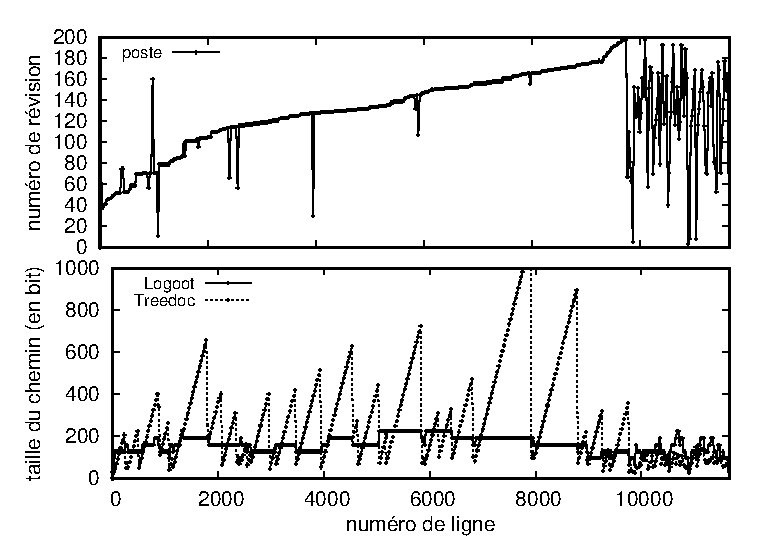
\includegraphics[width=0.8\textwidth]{img/lseq/motivationposte.eps}}
  \hspace{10pt}
  \subfloat[Document Wikipédia principalement édité au début.]
  [\label{repl:img:motivationsA}Document Wikipédia de petite taille
  principalement édité au début.]
  {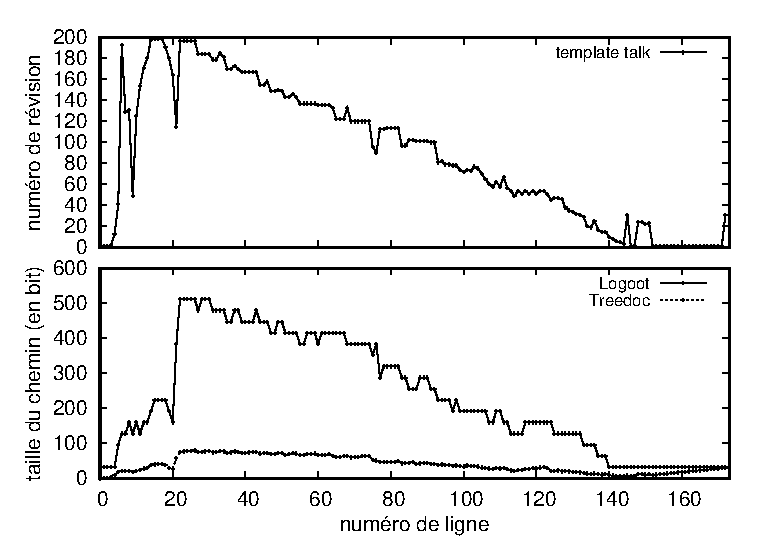
\includegraphics[width=0.8\textwidth]{img/lseq/motivationtemplatetalk.eps}}
  \caption{\label{repl:img:motivations} Taille du chemin alloué pour chaque
    ligne du document. L'axe des abcisses montre le numéro de la ligne
    concernée. L'axe des ordonnées de la partie haute de la figure montre l'âge
    de la ligne. L'axe des ordonnées de la partie basse de la figure montre la
    taille binaire du chemin alloué.}
\end{figure*}

L'encyclopédie Wikipédia répertorie des millions d'articles écrits
collaborativement par sa communauté. Un utilisateur, enregistré ou non, peut
lire un article, et s'il le souhaite, en modifier le contenu. Lorsque ses
modifications sont achevées, il les soumet à Wikipédia. Deux issues possibles :
\begin{inparaenum}[(i)]
\item La contribution est acceptée et sera visible de tous ou
\item la contribution est rejetée car un autre utilisateur a effectué une
  modification en concurrence et l'a soumise en premier. Il faut alors réviser
  la version rejetée afin de l'adapter à la version la plus à jour avant de
  resoumettre si nécessaire.
\end{inparaenum}
Wikipédia garde l'historique des modifications apportées à tous les articles
depuis leur création. Nous sommes alors à même de rejouer les éditions --
nommées révision -- dans l'ordre où elles ont été effectuées. Toutefois, la
concurrence qui pourrait exister dans une édition en temps réelle est effacée
par le processus d'édition même. D'autre part, la granularité est fixée à la
ligne. En cela, les simulations sur corpus Wikipédia diffèrent légèrement de la
réalité.

\begin{itemize}
\item [\textbf{Objectif :}] Montrer que ni Logoot ni Treedoc ne parviennent à
  fournir des identifiants dont la taille soit satisfaisante quel que soit le
  document.
\item [\textbf{Description :}] Logoot est configuré avec une base
  $2^{32}$. Treedoc est configuré pour utiliser sa méthode originelle -- son
  autre heuristique revenant plus ou moins à la stratégie de Logoot. Les
  documents considérés sont des articles extrait de Wikipédia joués sur 200
  révisions. L'un des articles possède à la fin plus de 10k lignes
  principalement ajoutées en fin
  d'article\footnote{\url{https://fr.wikipedia.org/wiki/Liste_des_bureaux_de_poste_français_classés_par_oblitération_Petits_Chiffres}}. L'autre
  article possède seulement 200 lignes mais est principalement édité en
  tête\footnote{\url{https://en.wikipedia.org/wiki/Template_talk:Did_you_know}}.
\item [\textbf{Résultat :}] Les figures~\ref{repl:img:motivationsA}
  et~\ref{repl:img:motivationsB} montrent la taille de l'identifiant associé à
  chaque ligne. Nous observons que Treedoc possède des chemins qui augmentent
  très vite quel que soit le type d'édition. Lorsque le nombre d'insertions
  successives est très grand (cf. figure~\ref{repl:img:motivationsA}) les
  chemins atteignent des tailles prohibitives. Dans ce cas, Logoot se comporte
  mieux. En revanche, dans le cadre de l'édition en tête, Logoot alloue des
  chemins de taille dramatiquement haute et en perpétuelle hausse.
\item [\textbf{Explication :}] Dans les deux types d'édition, Treedoc et Logoot
  allouent des identifiants dont la compléxité est linéaire. Ainsi, plus les
  insertions se succèdent, plus l'arbre est déséquilibré, plus la taille du
  chemin augmente. Mais comme la granularité des chemins Treedoc est binaire
  ($\mathcal{P}\in \mathbb{N}_{<2}.\mathbb{N}_{<2}\ldots\mathbb{N}_{<2}$), cela
  lui permet de conserver des chemins plus petits que ceux de Logoot dans le
  cadre du document édité en tête. D'un autre coté, Logoot a conçu sa stratégie
  pour l'édition en fin. Dès lors, si le comportement suit cette hypothèse, les
  identifiants grossissent par palliers, linéairement certes, mais lentement. En
  revanche, lorsque le comportement d'édition ne coopère pas, les identifiants
  grimpent très rapidement -- comme cela serait le cas avec la seconde
  heuristique de Treedoc.
\end{itemize}

%% Conclusion

%%% Local Variables:
%%% mode: latex
%%% TeX-master: "../../paper"
%%% End:
